\section{Experiments}
\label{sec:experiments}

\subsection{Setup}
    \label{sec:setup}

    \textbf{Platform and timing protocol.}
    All codec experiments are conducted on NVIDIA H200 GPUs. We report compression and decompression throughput in GB/s, where the byte count is the uncompressed native tensor size. Each codec benchmark first verifies bitwise round-trip correctness and then times repeated GPU executions after warm-up. For the baseline comparison, all methods operate on real BF16 activation tensors assembled as two-dimensional KV blocks. For transfer studies, we compose measured \splitzip encode/decode time, measured GPU host-device DMA time, and a staged layer-pipeline transfer model. The transport modes are CPU-RDMA at 376~Gb/s and RoCE 4$\times$200G at 700~Gb/s effective payload bandwidth. The breakdown uses additive sequential accounting. All codec throughput measurements were taken 10 times, and we report the average value.
    
    \textbf{Datasets and workloads.}
    Transfer workloads use authentic BF16 KV blocks extracted from one 1024-token forward pass per model and then assembled to target sequence lengths. We evaluate Llama-3-8B and Qwen3-30B-A3B from 512 to 64K tokens under both transport modes. For Qwen3-32B, we measure the codec throughput, compression ratio, and transmission breakdown using the chunk-local implementation with chunk size 1024. The batch size here is consistently 1. Since we flatten all activation values into a single tensor for processing, cases where the batch size is not 1 are equivalent to the scenario involving longer sequences. FP8 experiments also use Qwen3-32B and evaluate exact compression of native E4M3 and E5M2 tensors from 1K to 64K tokens. For all experiments, we calibrate the BF16 top-16 codebook on WikiText-2\cite{merity2016wikitext2} training subset.
    
    \textbf{Baselines and ablations.}
    For BF16 codec comparison, we compare nvCOMP LZ4\cite{nvidia2026nvcomp}, DFloat11\cite{dfloat11}, ZipNN\cite{zipnn}, and our \splitzip. For transfer-time studies, the native baseline moves raw BF16 or FP8 cache bytes, while \splitzip performs encode, compressed transfer, and decode. We further ablate BF16 top-8 3-bit coding versus top-16 4-bit coding, explicit escape-position storage versus sentinel-only escape discovery, pre-calibrated versus dynamic top-16 codebooks, and calibration granularity and generalizability. Ablation Experiments are on Qwen3-32B KV values.



\subsection{Results}
\label{sec:exp_results}

    \begin{figure}[t]
        \centering
        
\includegraphics[width=\textwidth]{figure/baseline_comparison.pdf}
        \caption{
        Codec-level comparison on real BF16 activation tensors.
        SplitZip achieves a competitive compression ratio while substantially improving both compression and decompression throughput over existing lossless compressors.
        }
        \label{fig:baseline_comparison}
        \vspace{-1.2em}
    \end{figure}
    
    \paragraph{Codec-level performance.}
    Figure~\ref{fig:baseline_comparison} compares SplitZip with existing lossless compressors.
    SplitZip achieves a competitive compression ratio, although it is not the highest-ratio method among the baselines.
    Its main advantage is codec throughput.
    For compression, SplitZip is $32.5\times$ faster than nvCOMP LZ4, $379\times$ faster than ZipNN and about $1.0\times 10^5$ faster than DFloat11.
    For decompression, SplitZip is $12.9\times$ faster than nvCOMP LZ4, $1069\times$ faster than ZipNN and $3.8\times$ faster than DFloat11.
    These results show that SplitZip sacrifices a modest amount of compression ratio in exchange for substantially higher codec throughput, which is critical when compression and decompression lie on the serving critical path.

    This throughput advantage comes from SplitZip's GPU-friendly codec design.
    SplitZip uses fixed-length exponent coding, regular bit manipulation, small lookup tables, and sparse escape correction, all of which map well to massively parallel GPU execution.
    As a result, compression and decompression can exploit otherwise underutilized GPU compute resources during KV-cache transfer.
    In contrast, DFloat11 and ZipNN perform compression on the CPU, making their compression throughput insufficient for online KV-cache transfer.
    Moreover, their Huffman-based variable-length coding introduces sequential dependencies during decoding, which limits parallelism and prevents decompression from reaching very high throughput.
    SplitZip instead targets KV-cache communication directly: it preserves a simple dense GPU path for the common case and isolates rare values into a lightweight escape stream.
        
    
    \begin{figure}[t]
        \centering
        
\includegraphics[width=\textwidth]{figure/transfer_time_vs_seq_len.pdf}
        \caption{
        End-to-end KV-cache transfer time across sequence lengths, models, and network settings.
        The dashed red line denotes the entropy-based theoretical optimum, ignoring encode/decode overhead and practical implementation constraints such as fixed-width bit alignment.
        }
        \label{fig:transfer_time_vs_seq_len}
        \vspace{-1.0em}
    \end{figure}
    
    \paragraph{Transfer time across sequence lengths.}
    Figure~\ref{fig:transfer_time_vs_seq_len} reports end-to-end transfer time for Llama-3-8B and Qwen3-30B-A3B under CPU-RDMA and RoCE $4\times200$G settings.
    The results for \splitzip presented here \textit{take encoding and decoding overhead into account}.
    The dashed red curve shows the zero-overhead theoretical optimum:
    \[
        T_{\mathrm{opt}} = \frac{T_{\mathrm{native}}}{\rho},
    \]
    where $T_{\mathrm{native}}$ is the native BF16 transfer time and $\rho$ is the entropy-based theoretical compression ratio.
    This represents the best possible transfer time if compression only reduced the payload size and introduced no codec overhead.
    
    For short sequences, SplitZip can be slower than native transfer because the KV-cache payload is small and codec overhead is not fully amortized.
    As sequence length increases, transfer time dominates and SplitZip becomes beneficial.
    For Llama-3-8B, SplitZip starts to outperform native transfer from sequence length $2$K.
    At $64$K, it achieves $1.326\times$ speedup under CPU-RDMA and $1.324\times$ speedup under RoCE $4\times200$G.
    For Qwen3-30B-A3B, SplitZip becomes beneficial from sequence length $4$K.
    At $64$K, it reaches $1.305\times$ speedup under CPU-RDMA and $1.273\times$ speedup under RoCE $4\times200$G.
    At long sequence lengths, the SplitZip curves closely follow the theoretical optimum, indicating that most of the compression benefit is preserved despite encode and decode overhead.

    One subtle point is that the speedup on Llama-3-8B at $64$K slightly exceeds the SplitZip compression ratio reported in Figure~\ref{fig:baseline_comparison}. 
    This is because Figure~\ref{fig:baseline_comparison} measures the codec-level compression ratio on Qwen activation tensors, while the Llama-3-8B KV activations have lower exponent entropy and fewer escape values.
    As a result, SplitZip obtains a slightly higher effective compression ratio on Llama-3-8B, allowing the end-to-end speedup to exceed the ratio shown in the codec-level comparison.
    By contrast, on Qwen3-30B-A3B, even at $64$K context length, the remaining encode and decode overhead still prevents SplitZip from exactly reaching the zero-overhead theoretical optimum.
    The resulting speedup remains within about $0.015\times$--$0.047\times$ of the theoretical curve, showing the importance of pipeline execution and transfer.
    
    \begin{figure}[t]
        \centering
        
\includegraphics[width=\textwidth]{figure/qwen32_transmission_breakdown.pdf}
        \caption{
        Transmission-time breakdown on Qwen3-32B under RoCE $4\times200$G.
        Native transfer sends the raw BF16 KV cache, while SplitZip consists of encoding, compressed transfer, and decoding.
        }
        \label{fig:qwen32_transmission_breakdown}
        \vspace{-1.0em}
    \end{figure}
    
    \paragraph{Transmission-time breakdown.}
    Figure~\ref{fig:qwen32_transmission_breakdown} further breaks down the Qwen3-32B transfer time under RoCE $4\times200$G.
    This breakdown uses additive accounting for encode, compressed transfer, and decode time.
    At sequence length $2$K, SplitZip slightly reduces transfer time from $56.5$~ms to $53.1$~ms.
    However, the advantage increases with sequence length.
    At $16$K, SplitZip reduces transfer time from $441.4$~ms to $353.8$~ms.
    At $64$K, it reduces transfer time from $1749.3$~ms to $1397.0$~ms.
    In this long-context regime, compressed transfer accounts for $92.9\%$ of the SplitZip time, while encoding and decoding account for only $5.7\%$ and $1.4\%$, respectively.
    This confirms that SplitZip keeps codec overhead small enough for long-context KV-cache transfer to remain primarily communication-bound.

    \paragraph{FP8 Result.}
    \begin{figure*}[t]
    \centering

    \begin{minipage}[t]{0.4\textwidth}
        \vspace{0pt}
        \centering
        \captionof{table}{FP8 codec results.}
        \label{tab:fp8_exact_results}
        \footnotesize
        \setlength{\tabcolsep}{2.5pt}
        \renewcommand{\arraystretch}{1.12}
        \begin{tabular}{@{}lccc@{}}
            \toprule
            \textbf{Metric}
            & \textbf{E4M3}
            & \textbf{E5M2}
            & \textbf{E5M2} \\
            & \textbf{Top-8}
            & \textbf{Top-8}
            & \textbf{Top-16} \\
            \midrule
            Coverage
            & 92.17\%
            & 92.28\%
            & 99.84\% \\
            Ratio vs. FP8
            & $0.933\times$
            & $1.049\times$
            & $1.136\times$ \\
            Ratio vs. BF16
            & $1.866\times$
            & $2.097\times$
            & $2.273\times$ \\
            Encode(GB/s)
            & 219.6$\pm$1.5
            & 221.6$\pm$14.6
            & 249.7$\pm$0.8 \\
            Decode(GB/s)
            & 366.9$\pm$2.5
            & 340.8$\pm$0.9
            & 564.9$\pm$6.5 \\
            Escape rate
            & 7.83\%
            & 7.72\%
            & 0.16\% \\
            \bottomrule
        \end{tabular}
    \end{minipage}
    \hfill
    \begin{minipage}[t]{0.5\textwidth}
        \vspace{0pt}
        \centering
        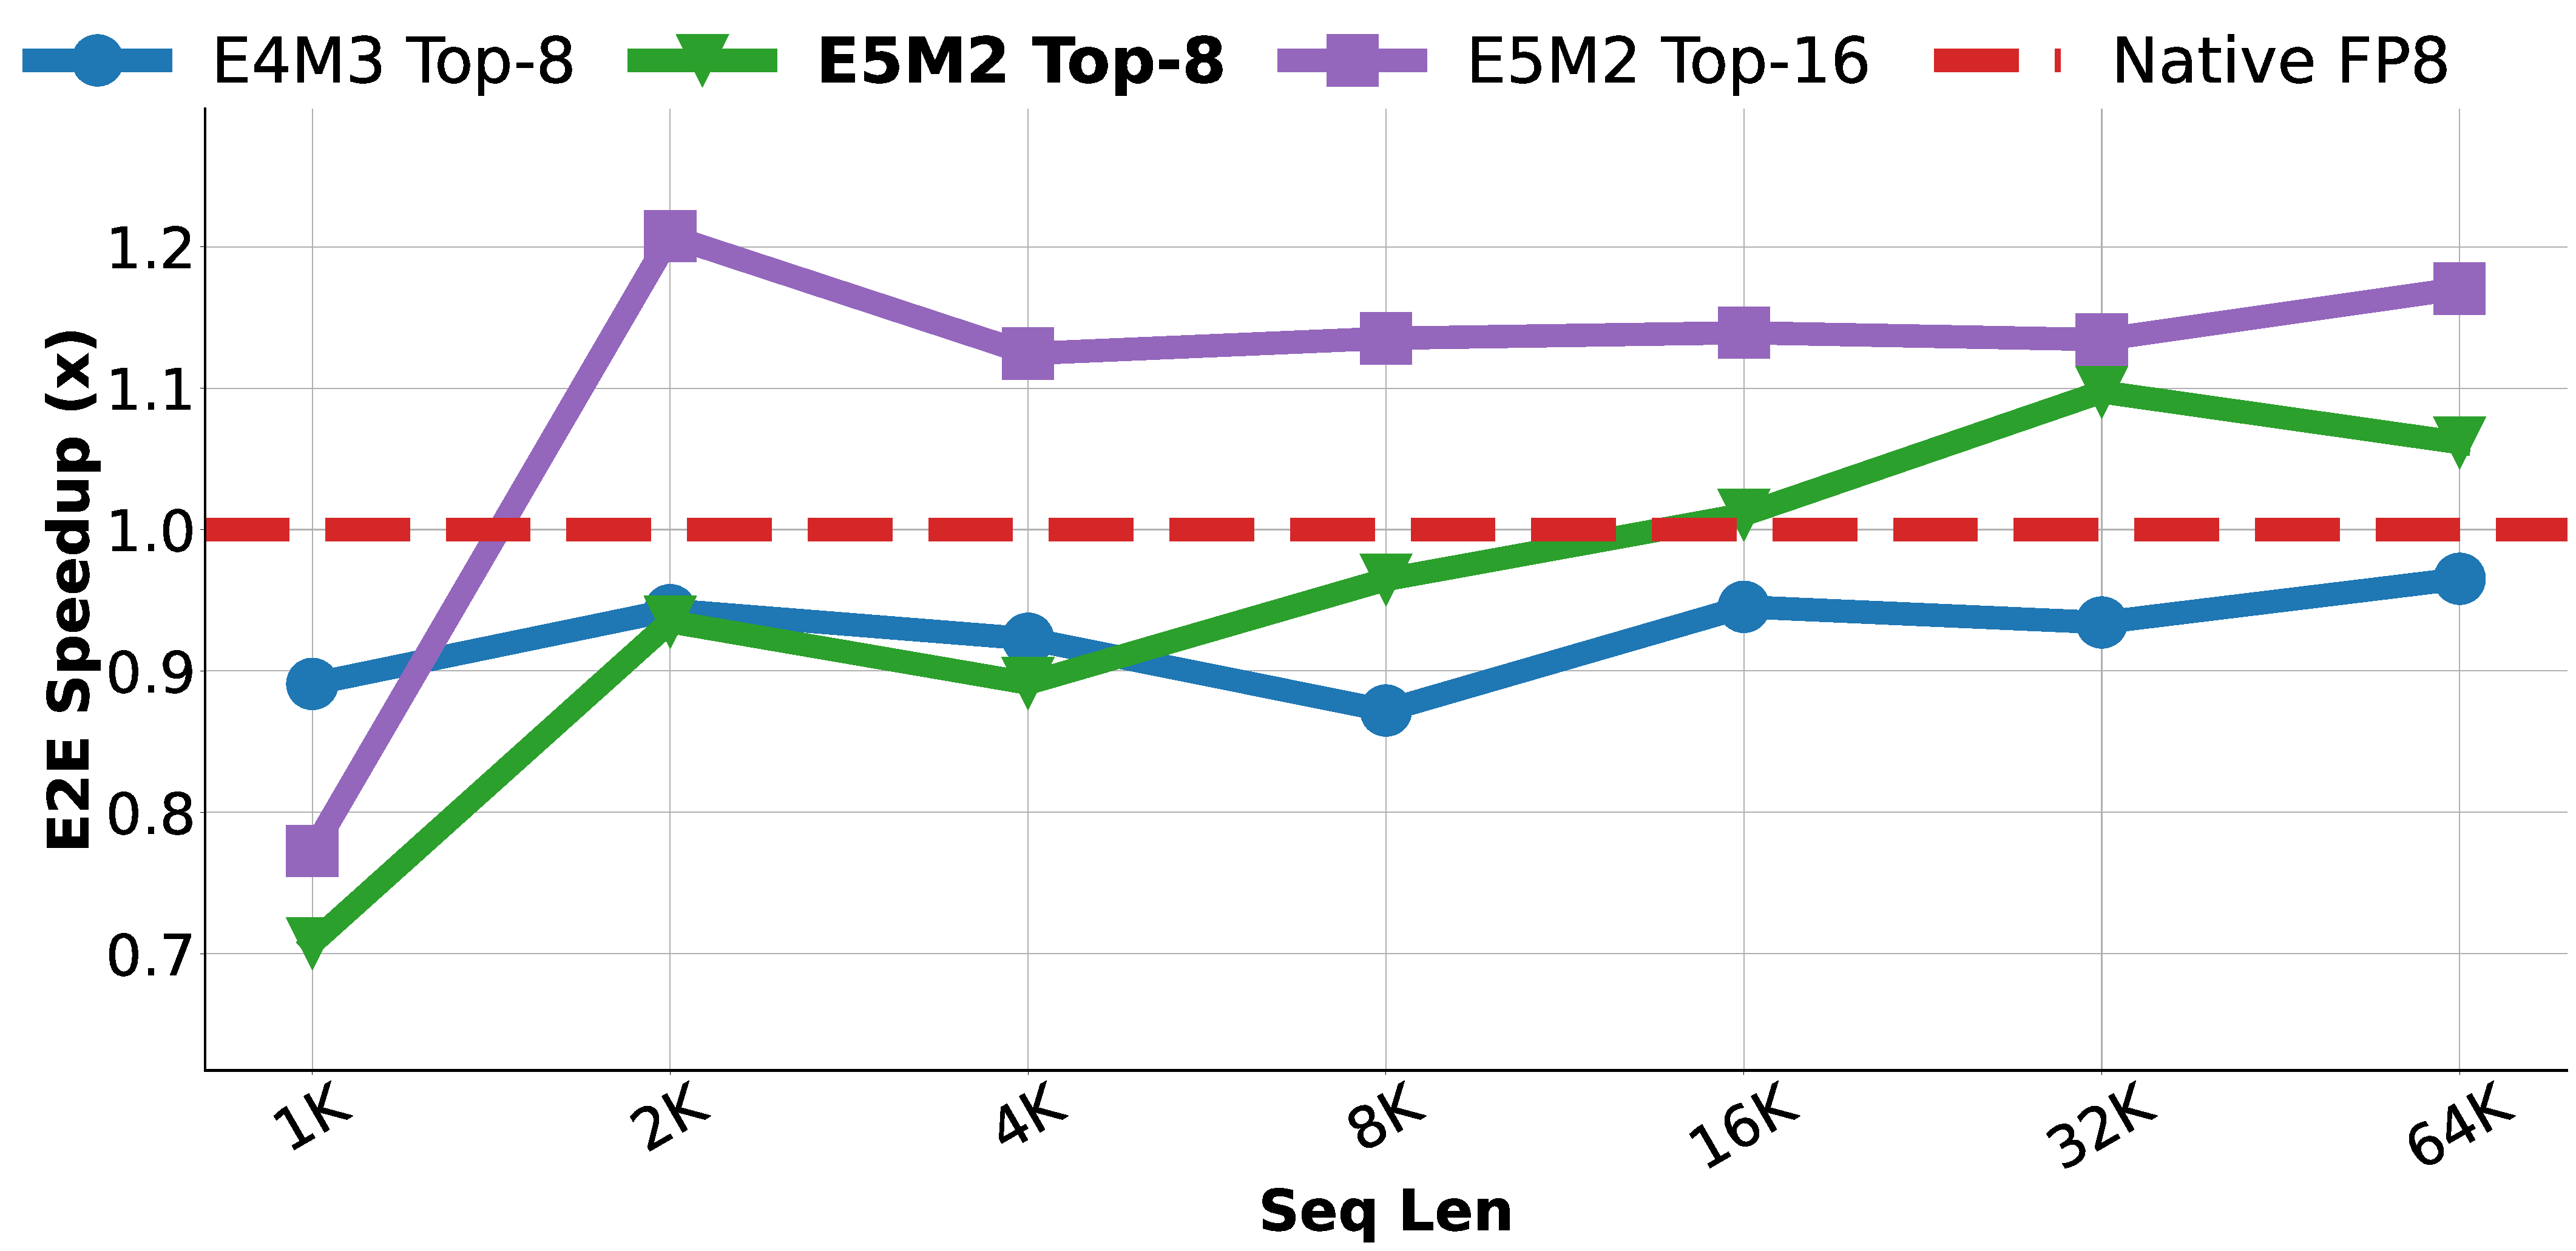
\includegraphics[width=\linewidth]{lossless-paper/figure/fp8_e2e_speedup_vs_seq_len.pdf}
        \vspace{-1.5em}
        \captionof{figure}{
        FP8 end-to-end transfer time on Qwen3-32B under RoCE $4\times200$G.
        }
        \label{fig:fp8_transfer_time}
    \end{minipage}
\vspace{-2em}
\end{figure*}


    Table~\ref{tab:fp8_exact_results} and Figure~\ref{fig:fp8_transfer_time} report the FP8 results of SplitZip.
    Since FP8 already halves the KV-cache size compared with BF16, the remaining lossless compression opportunity is smaller.
    Nevertheless, SplitZip still provides additional compression over native FP8.
    E4M3 Top-8 expands the payload because its exponent field is already compact and the escape metadata is too large for this distribution.
    E5M2 offers more redundancy, and the Top-16 variant achieves both the highest compression ratio and the lowest escape rate.
    
    The lower escape rate of E5M2 Top-16 also improves throughput: it reaches 249.7~GB/s encoding and 564.9~GB/s decoding, compared with 221.6~GB/s and 340.8~GB/s for E5M2 Top-8.
    This mirrors the BF16 trend that reducing escapes is more important than shrinking the dense code width when sparse correction dominates the tail cost.
    
    For end-to-end transfer, all FP8 variants are slower than native FP8 at short sequence lengths because codec overhead dominates.
    As the sequence length increases, transfer time becomes the bottleneck and SplitZip begins to improve performance.
    E5M2 Top-16 reaches positive speedup earlier due to its high coverage and low escape rate, and reaches $1.17\times$ speedup at 64K.
    E5M2 Top-8 requires longer contexts to amortize its higher escape overhead and reaches $1.06\times$ at 64K, while E4M3 Top-8 remains slower than native FP8.
    This suggests that Top-16 is the preferable FP8 setting for the measured Qwen3-32B workload.


\subsection{Ablation Study}
    \subsubsection{Ablation on Top-$k$ Exponent Coding}
\label{sec:ablation_topk}

\begin{wraptable}{r}{0.35\linewidth}
    \vspace{-1.2em}
    \centering
    \caption{Top-$k$ exponent coding.}
    \label{tab:ablation_topk}
    \footnotesize
    \setlength{\tabcolsep}{4pt}
    \renewcommand{\arraystretch}{1.08}
    \begin{tabular}{lcc}
        \toprule
        \textbf{Metric} & \textbf{Top-8} & \textbf{Top-16} \\
        \midrule
        Code width & 3-bit & 4-bit \\
        Coverage & 95.62\% & 99.67\% \\
        Ratio & $1.364\times$ & $1.316\times$ \\
        Encode(GB/s) & 272.6 & 329.9 \\
        Decode(GB/s) & 492.2 & 1263.3 \\
        Escape rate & 4.38\% & 0.33\% \\
        \bottomrule
    \end{tabular}
    \vspace{-1.7em}
\end{wraptable}

Table~\ref{tab:ablation_topk} compares Top-8 3-bit coding with Top-16 4-bit coding.
Top-8 slightly improves the compression ratio from $1.316\times$ to $1.364\times$, but substantially reduces throughput.
Top-16 is $1.21\times$ faster in encoding and $2.57\times$ faster in decoding.

The slowdown of Top-8 comes from both higher escape overhead and less GPU-friendly packing.
Reducing the codebook from 16 to 8 entries lowers coverage from 99.67\% to 95.62\%, increasing the escape rate from 0.33\% to 4.38\%.
This nearly $13\times$ higher escape rate increases memory-intensive escape collection and sparse overwrite costs.
In addition, 3-bit codes do not align naturally with byte-oriented GPU operations, unlike 4-bit codes where two exponents form one byte.
The FP8 results in Table~\ref{tab:fp8_exact_results} show the same trend: lower-bit exponent coding does not necessarily improve end-to-end performance.
    \subsubsection{Ablation on Calibration Dataset}
\label{sec:ablation_calibration}

\begin{wraptable}{r}{0.4\linewidth}
    \vspace{-1.2em}
    \centering
    \caption{Cross-dataset calibration coverage. Dataset A is WikiText-2 train.}
    \label{tab:ablation_calibration}
    \scriptsize
    \setlength{\tabcolsep}{5pt}
    \renewcommand{\arraystretch}{1.08}
    \begin{tabular}{llcc}
        \toprule
        \textbf{Eval set} & \textbf{Domain} & \textbf{A$\rightarrow$B} & \textbf{B$\rightarrow$B} \\
        \midrule
        WikiText-2 & Language & 99.65\% & 99.65\% \\
        HumanEval & Code & 99.66\% & 99.66\% \\
        GSM8K & Math & 99.64\% & 99.64\% \\
        MMLU & Knowledge & 99.63\% & 99.63\% \\
        PTB & Language & 99.55\% & 99.58\% \\
        \bottomrule
    \end{tabular}
    \vspace{-1.7em}
\end{wraptable}

SplitZip uses a calibrated top-16 exponent codebook to avoid online histogram construction.
To test whether this codebook is dataset-specific, we calibrate on WikiText-2 train and evaluate coverage on datasets from different domains.
Table~\ref{tab:ablation_calibration} compares cross-dataset calibration, denoted A$\rightarrow$B, with oracle calibration on each target dataset, denoted B$\rightarrow$B.

The calibrated exponent set generalizes well.
Coverage remains between 99.55\% and 99.66\% across all evaluated datasets, and matches the oracle result on WikiText-2 test, HumanEval~\cite{chen2021humaneval}, GSM8K~\cite{cobbe2021gsm8k}, and MMLU~\cite{hendrycks2021mmlu}.
Even on PTB~\cite{zhou2020ptb}, the gap is only 0.03 percentage points.
This shows that high-frequency KV-cache exponents are stable across domains, enabling SplitZip to use a fixed offline codebook.

    \subsubsection{Ablation on Calibration Granularity}
\label{sec:ablation_granularity}

\begin{wraptable}[6]{r}{0.40\linewidth}
    \vspace{-1.6em}
    \centering
    \caption{Calibration granularity ablation.}
    \label{tab:ablation_granularity}
    \scriptsize
    \setlength{\tabcolsep}{5pt}
    \renewcommand{\arraystretch}{1.02}
    \begin{tabular}{lccc}
        \toprule
        \textbf{Metric} & \textbf{Tensor} & \textbf{Token} & \textbf{Channel} \\
        \midrule
        Coverage & 99.60\% & 99.74\% & 99.98\% \\
        Compression & $1.323\times$ & $1.322\times$ & $1.329\times$ \\
        Encode(GB/s) & 93.9 & 0.082 & 0.020 \\
        Decode(GB/s) & 222.2 & 0.173 & 0.060 \\
        \bottomrule
    \end{tabular}
    \vspace{-1.0em}
\end{wraptable}

Some prior compression designs use finer-grained codebooks to improve locality, compression ratio, or parallelism.
We evaluate this idea on per-tensor, per-token and per-channel codebooks.

Table~\ref{tab:ablation_granularity} shows that finer-grained calibration increases top-16 coverage, reaching 99.98\% with per-channel codebooks.
However, the projected compression ratio improves only marginally, from $1.323\times$ to $1.329\times$.
In contrast, throughput drops by several orders of magnitude: per-token and per-channel calibration both fall from hundreds of GB/s to sub-GB/s performance.
This is because fine-grained calibration requires many small codebooks, introducing extra storage, irregular lookup patterns, and more complex GPU execution.
Therefore, SplitZip uses a single global codebook, which preserves nearly the same compression ratio while maintaining a simple and high-throughput dense path.
    \subsubsection{Ablation on Escape-Position Metadata}
\label{sec:ablation_escape_position}

\begin{wraptable}{r}{0.4\linewidth}
    \vspace{-1.4em}
    \centering
    \caption{Escape-position ablation.}

    \label{tab:ablation_escape_position}
    \scriptsize
    \setlength{\tabcolsep}{6pt}
    \renewcommand{\arraystretch}{1.08}
    \begin{tabular}{lcc}
        \toprule
        \textbf{Metric} & \textbf{Top-16 + Pos.} & \textbf{Top-15 + Sent.} \\
        \midrule
        Coverage & 99.84\% & 99.73\% \\
        Escape rate & 0.16\% & 0.27\% \\
        Ratio & $1.324\times$ & $1.331\times$ \\
        Encode(GB/s) & 435.3  & 396.0  \\
        Decode(GB/s) & 1763.8  & 620.8  \\
        \bottomrule
    \end{tabular}
    \vspace{-1.4em}
\end{wraptable}

We also study whether SplitZip should explicitly store escape positions or reserve one code as an escape sentinel.
The sentinel design uses only 15 frequent exponent values and reserves the remaining 4-bit code to mark escaped elements.
This avoids storing explicit chunk-local positions and therefore slightly improves the compression ratio, from $1.324\times$ to $1.331\times$.
However, this metadata saving comes at a large decoding cost.

As shown in Table~\ref{tab:ablation_escape_position}, the Top-15 sentinel design reduces decode throughput from 1763.8~GB/s to 620.8~GB/s, a $2.84\times$ slowdown.
The reason is that the decoder can no longer treat all 4-bit codes uniformly.
It must inspect the dense code stream to identify sentinel values and then merge escaped exponents back into the output, introducing irregular control flow and memory access.
In contrast, the Top-16 design decodes every element through the same dense lookup path and applies rare escape corrections through a separate sparse overwrite.
Although this requires explicit position metadata, the escape rate is only 0.16\%, making the metadata overhead small.
Therefore, SplitZip chooses Top-16 coding with explicit escape positions to prioritize decoding throughput and GPU regularity over a marginal compression-ratio gain.

    \subsubsection{Ablation on Pre-Calibration}
\label{sec:ablation_precalibration}

\begin{wraptable}[8]{r}{0.40\linewidth}
    \vspace{-1.2em}
    \centering
    \caption{Pre-calibration ablation.}
    \label{tab:ablation_precalibration}
    \scriptsize
    \setlength{\tabcolsep}{8pt}
    \renewcommand{\arraystretch}{1.08}
    \begin{tabular}{lcc}
        \toprule
        \textbf{Metric} & \textbf{Pre-calib.} & \textbf{Dynamic} \\
        \midrule
        Ratio & $1.324\times$ & $1.324\times$ \\
        Escape rate & 0.16\% & 0.16\% \\
        Encode(GB/s) & 430.1 & 80.7 \\
        Decode(GB/s) & 1745.1 & 1779.1 \\
        \bottomrule
    \end{tabular}
    \vspace{-1.5em}
\end{wraptable}

We compare SplitZip's offline pre-calibrated codebook with a dynamic Top-16 variant that rebuilds the exponent codebook for each input.
As shown in Table~\ref{tab:ablation_precalibration}, dynamic calibration achieves the same compression ratio and escape rate as the pre-calibrated design, and decode throughput is almost unchanged.
However, it substantially slows down online compression: encode throughput drops from 430.1~GB/s to 80.7~GB/s, $5.3\times$ slower, because the dynamic variant adds an online histogram and top-$k$ selection pass.

